\documentclass[conference]{IEEEtran}
\usepackage{cite}
\usepackage{amsmath,amssymb}
\usepackage{graphicx}
\usepackage{booktabs,array}
\usepackage{microtype}
\usepackage{url}
\usepackage[hidelinks]{hyperref}
\graphicspath{{../figures/}}
% Generated from review/audit.py. Do not edit numerical rows manually.
\newcommand{\ReviewEnergyRows}{
3B & Primary & 195.6 & 0.091 & 0.078--0.093 \\
3B & Repeat & 196.4 & 0.091 & 0.078--0.094 \\
8B & Primary & 101.8 & 0.19 & 0.18--0.19 \\
8B & Repeat & 102.5 & 0.19 & 0.17--0.20 \\}
\newcommand{\ReviewHostRows}{
3B & 0.091 & 0.10 & 0.12 & 0.13 & 0.15 \\
8B & 0.19 & 0.22 & 0.24 & 0.27 & 0.31 \\}
\newcommand{\ReviewAmdRows}{
Ministral-3 3B & 78.4 & 2711 & 5.7 & 0.050 \\
Ministral-3 8B & 37.8 & 1161 & 7.4 & 0.055 \\
Qwen3.8 27B & 13.8 & 341 & 233.2 & 0.078 \\}
\newcommand{\ReviewIntegratedRequests}{38}
\newcommand{\ReviewRawRepetitions}{68}
\newcommand{\ReviewLadderRows}{
AMD & \texttt{private-3.1b-q8:latest} & 3.285 & 59.77 & 76.7 & Summary \\
AMD & \texttt{private-7.6b-vlm-q8:latest} & 9.453 & 28.62 & 105.7 & Summary \\
AMD & \texttt{gemma4:26b} & 17.988 & 58.34 & 409.9 & Summary \\
AMD & \texttt{gemma4:e4b} & 9.608 & 56.42 & 211.8 & Summary \\
AMD & \texttt{ministral-3:3b} & 2.954 & 78.62 & 90.7 & Summary \\
AMD & \texttt{ministral-3:8b} & 6.022 & 37.81 & 88.9 & Summary \\
AMD & \texttt{muse-glimmer:30b} & 18.157 & 12.46 & 88.4 & Summary \\
AMD & \texttt{qwen3.6:latest} & 23.938 & 62.20 & 581.6 & Summary \\
AMD & \texttt{qwen3.8:27b} & 17.742 & 19.63 & 136.0 & Summary \\
RTX & \texttt{ministral-3:3b} & 2.954 & 199.28 & 87.6 & Raw \\
RTX & \texttt{ministral-3:8b} & 6.022 & 103.96 & 93.2 & Raw \\
RTX & \texttt{qwen3:4b} & 2.497 & 169.92 & 63.1 & Raw \\}

\hypersetup{
pdftitle={Right-Sized AI at the Edge: Reproducible Measurements and Conditional Sustainability Analysis},
pdfauthor={AutoYou Research},
pdfsubject={Working paper; revised 20 September 2026; not peer reviewed}}
\begin{document}
\title{Right-Sized AI at the Edge:\\
Reproducible Measurements and Conditional\\
Sustainability Analysis}
\author{\IEEEauthorblockN{AutoYou Research}
\IEEEauthorblockA{%
\texttt{research@autoyou.me}\\
Working paper, revised 20 September 2026. Not peer reviewed.}}
\maketitle
\pagestyle{plain}
\thispagestyle{plain}

\begin{abstract}
Moving language-model inference to consumer hardware can change its energy,
carbon, water, and financial costs, but a smaller per-request number does not
establish a saving at equivalent service quality. We examine archived
single-stream measurements from a Radeon 8060S system and an RTX 5070 system
and provide a boundary-explicit accounting model. An independent implementation
replays 68 stored generation repetitions, including 38 requests with
bracketed board-power telemetry. At 499 input and 300 output tokens, the
RTX 5070 records median request-window board energies of 0.091 Wh and 0.19 Wh
for the recorded Ministral-3 3B and 8B builds. A second session on the same
machine gives the same rounded medians. Assuming 60 W of additional host
power and 90\% supply efficiency changes the primary-session estimates to
0.13 Wh and 0.27 Wh; these are scenarios, not wall-meter observations.
A twelve-row throughput/file-size comparison demonstrates why this
proxy cannot be read as measured memory-bandwidth utilization.
We derive accounting expressions that include failed local attempts,
cloud fallback, and a common demand-growth factor across footprint metrics.
The records do not establish quality-matched cloud displacement,
population-wide task coverage, total cost of ownership, or fleet-scale
environmental savings. The contribution is a reproducible deployment case
study and a specification of the additional evidence needed for a credible
edge-versus-cloud sustainability claim.
\end{abstract}
\begin{IEEEkeywords}
edge inference, energy measurement, carbon accounting, water consumption,
small language models, reproducibility
\end{IEEEkeywords}

\section{Introduction}
Whether an inference deployment is sustainable depends on the service it
delivers and the boundary used to count its resources. Board energy,
whole-computer electricity, data-centre electricity, and life-cycle emissions
are different quantities. A short local response is not an interchangeable
substitute for a long cloud response without a task-level quality test.

The International Energy Agency's 2025 base case projects approximately
945 TWh of \emph{all data-centre} electricity demand in 2030
\cite{iea2025}. That motivates careful measurement; it does not supply a
direct estimate of the fraction that consumer inference could replace.
We therefore ask what can be established from single-stream consumer
deployment records, and what remains conditional when they enter an
environmental comparison.

The supplied artifact contains measurements recorded in September 2026 on
two Windows 11 machines. We retain their device and model labels as
recorded, without treating a runtime tag as an immutable model identifier
or independent verification of a vendor release. No new hardware experiment
was performed for this revision.

Our contributions are:
\begin{enumerate}
\item an arithmetic replay of stored timings and power traces, distinguishing
raw observations from aggregate-only records;
\item request-window energy results with consistent board, host, and supply
boundaries, and a cautionary analysis of file-size proxies;
\item conditional accounting that charges local failures and uses one
demand-growth assumption for energy, water, carbon, and cost.
\end{enumerate}
We do not claim a new inference algorithm, the first consumer-GPU benchmark,
or an experimentally demonstrated reduction in cloud impact.

\section{Related Work and Comparison Boundaries}
Elsworth et al.\ measure production AI serving at Google and report
0.24 Wh for a median Gemini Apps text prompt, accounting for accelerator,
host, idle-capacity, and facility energy \cite{elsworth2025}.
Their production population is not the prompt used here.
Jegham et al.\ combine API performance with inferred infrastructure in an
environmental \emph{estimation} framework \cite{jegham2025}.
Their numbers are not direct wall-power readings from those providers.

Consumer inference is already studied. Knoop and Holtmann evaluate
consumer Blackwell deployments across models and configurations
\cite{knoop2026}. Tummalapalli et al.\ study sustained edge inference and
explicitly discuss inconsistent power-measurement boundaries across
platforms \cite{tummalapalli2026}. Our small case study complements these
works through replayable request traces and boundary sensitivity; it does
not supersede their broader evaluations. MLPerf Inference illustrates the
importance of explicit workload, scenario, and quality requirements
\cite{reddi2020mlperf}. This is not an MLPerf submission.

Belcak et al.\ motivate heterogeneous small/large-model agents
\cite{belcak2025}. Their Appendix B gives \emph{estimates} of replaceable
calls in three agent architectures, not a sampled estimate of local success
for our application. Luccioni et al.\ discuss rebound effects and the
limits of inferring societal impact from technical efficiency
\cite{luccioni2025}; that work does not calibrate a 15--25\% take-back rate
for this deployment. Water accounting must distinguish withdrawal from
consumption, and on-site cooling from electricity-generation impacts
\cite{li2025water}.

\section{Data and Methods}
\subsection{Deployment Records and Protocol}
The AMD records identify a Ryzen AI MAX+ 395 with Radeon 8060S graphics,
nominal 64 GiB system memory, and Ollama 0.33.2. The NVIDIA records identify
an RTX 5070, nominal 12 GiB graphics memory, an Intel Core i9-13900 host,
Ollama 0.33.3, and driver 610.47. These are recorded configurations, not
controlled comparisons of silicon architectures.

The harness uses a synthetic explanatory prompt, temperature zero, a fixed
seed, a 4096-token context setting, and a discarded warm-up.
Raw mode bypasses prompt templating \cite{ollamaapi2026}.
A varying prefix is placed before the prompt to reduce prefix-cache reuse.
These controls reduce a known confound; they do not prove that every
runtime cache is disabled. Loading and first-use initialization are
outside the warm request window.

Table~\ref{tab:corpus} identifies the six files. The primary and repeat
NVIDIA sessions retain seven repetitions per model, with 499 input tokens
and 300 generated tokens. Other files have different prompt lengths and
generation limits and are not pooled into those energy medians.
The two Ministral-3 tags describe Q4\_K\_M builds, with recorded parameter
labels of 3.8B and 8.9B. The short 3B and 8B labels below refer to their
runtime names.

\begin{table}[t]
\caption{Archived evidence. File names share the suffix \texttt{.json}.
Raw concerns main generation repetitions, not all auxiliary observations.}
\label{tab:corpus}
\centering\footnotesize
\setlength{\tabcolsep}{3pt}
\begin{tabular}{lrrrr}
\toprule
File stem & Models & Reps. & Output & Raw\\
\midrule
\texttt{amd-8060s-strixhalo} & 3 & 5 & 192 & Yes\\
\texttt{amd-8060s-strixhalo-ladder} & 9 & 7 & 128 & No\\
\texttt{rtx5070} & 2 & 5 & 192 & Yes\\
\texttt{rtx5070-study} & 2 & 7 & 300 & Yes\\
\texttt{rtx5070-replication} & 2 & 7 & 300 & Yes\\
\texttt{rtx5070-ladder} & 3 & 5 & 192 & Yes\\
\bottomrule
\end{tabular}
\end{table}

There are \ReviewRawRepetitions{} stored main-run repetitions.
The AMD ladder instead retains nine medians, ranges, and metadata records,
each reporting seven repetitions. Those underlying repetitions are
unavailable. Prefill sweeps also retain point medians rather than all
individual timing observations. Two AMD ladder model labels are anonymized
and their weights are not redistributed. Arithmetic checks and anonymized
tags do not establish independent reproducibility of those builds.

\subsection{Telemetry Integration}
For NVIDIA, the harness polls \texttt{power.draw.instant} through
\texttt{nvidia-smi}. NVIDIA describes this as the latest board-power
measurement, not a whole-system meter \cite{nvidiasmi2026}.
Samples carry request-relative timestamps and bracket the request window.

For samples $(t_i,P_i)$ in seconds and watts, define the linear interpolant
\begin{equation}
\widehat{P}(t)=P_i+
 \frac{P_{i+1}-P_i}{t_{i+1}-t_i}(t-t_i).
\end{equation}
For a request lasting $T$ seconds, board energy is
\begin{equation}
E_b=\frac{1}{3600}\int_0^T\widehat{P}(t)\,dt
\quad\text{in Wh}. \label{eq:board}
\end{equation}
The independent replay clips segments to $[0,T]$, rejects non-monotonic
or unbracketed traces, and checks serialized energy, mean power,
wall-window duration, token counts, and median throughput.
It does not import the original analytical model.

Repeated polling does not create independent sensor readings.
In the primary and repeat 300-token sessions, individual requests
contain only 3--4 distinct in-window power values for 3B and 6--7 for 8B.
These counts do not determine sensor accuracy or true update frequency.
Instrument latency, smoothing, and interpolation can bias short-window
estimates. We use two significant figures for energy as a conservative
reporting convention, not a calibrated uncertainty bound.

\subsection{Host and Supply Boundary}
For assumed non-GPU host DC power $P_h$ and supply efficiency $\eta$,
a request-window AC estimate is
\begin{equation}
E_{\mathrm{AC}}=\frac{E_b+P_hT/3600}{\eta}. \label{eq:wall}
\end{equation}
We evaluate $P_h\in\{0,30,60,100\}$ W with $\eta=0.90$.
Each run is transformed before taking the median; multiplying separate
medians is not generally equivalent. Even the zero-host scenario includes
supply loss and differs from the board-only value.
These host and efficiency values are assumptions, not measurements.
Display power, external networking, building cooling, and additional
keep-awake time are outside this table.

An incremental-energy claim requires an idle counterfactual at the
\emph{same} measurement boundary. Subtracting whole-desktop idle watts
from GPU-board watts is invalid. Already owning a device does not establish
zero incremental idle time or zero life-cycle impact.

\subsection{Timing Fits and File-Size Proxy}
Generation throughput is $\tau=n_o/t_{\mathrm{decode}}$, using
server-reported output count and decode duration. For each AMD model,
ordinary least squares fits four archived prompt-sweep medians:
\begin{equation}
\widehat{t}_{\mathrm{prefill}}(n_i)=a+bn_i,\qquad
\widehat{\beta}(n_i,n_o)=\frac{a+bn_i}{n_o/\tau}. \label{eq:prefill}
\end{equation}
$1/b$ describes a marginal fitted prefill rate, not end-to-end throughput.
$\widehat{\beta}(500,300)$ is a model-based projection within the swept
prompt range, not a measured 500/300-token AMD request.

The ladder statistic is
\begin{equation}
U_{\mathrm{file}}=\frac{\tau W_{\mathrm{file}}}{B_{\mathrm{ref}}}.
\label{eq:proxy}
\end{equation}
$W_{\mathrm{file}}$ is recorded decimal GB, and $B_{\mathrm{ref}}$ is a
nominal bandwidth reference, 256 GB/s for AMD and 672 GB/s for NVIDIA,
as recorded in the artifact. We do not measure sustainable bandwidth.
The numerator is \emph{not} measured memory traffic: a file can contain
inactive experts, vision components, metadata, and tensors accessed at
different frequencies. Cache reuse, quantization, runtime kernels, and
speculative decoding further affect the relationship.

\section{Results}
\subsection{Arithmetic Replay and Request Energy}
All \ReviewIntegratedRequests{} archived powered requests reproduce
serialized energy within $5.0\times10^{-7}$ Wh, consistent with rounding.
This demonstrates internal arithmetic consistency, not physical
calibration or authenticity. Likewise, $\bar{P}T=3600E_b$ is an identity
when $\bar{P}$ is derived from the same integral, not independent validation.

\begin{table}[t]
\caption{RTX 5070 board telemetry for 499 input and 300 output tokens.
Seven runs per row. Ranges are observed minima and maxima, not confidence
intervals.}
\label{tab:energy}
\centering\small
\setlength{\tabcolsep}{4pt}
\begin{tabular}{llrrr}
\toprule
Build & Session & Tok/s & Median Wh & Range Wh\\
\midrule
\ReviewEnergyRows
\bottomrule
\end{tabular}
\end{table}

Table~\ref{tab:energy} shows stable rounded medians across two sessions.
The file called replication is a repeat on the same machine and stack,
not replication by an independent laboratory. The primary 3B and 8B
window medians are approximately 1.62 and 3.11 s.
Across primary and repeat sessions, wall time minus reported prefill
and decode time ranges from about 26 to 72 ms. We do not attribute
that residual to one mechanism.

\begin{table}[t]
\caption{Primary-session energy in Wh. Board is measured via telemetry;
all AC columns are Eq.~\eqref{eq:wall} scenarios with $\eta=0.90$ and
the stated host DC power.}
\label{tab:host}
\centering\small
\setlength{\tabcolsep}{4pt}
\begin{tabular}{lrrrrr}
\toprule
Build & Board & AC: 0 W & AC: 30 W & AC: 60 W & AC: 100 W\\
\midrule
\ReviewHostRows
\bottomrule
\end{tabular}
\end{table}

At 60 W host power, modeled AC energy is 0.13 Wh for 3B and 0.27 Wh for
8B (Table~\ref{tab:host} and Fig.~\ref{fig:host}).
Neither can be compared directly to a production cloud median without
matching the task and service boundary. The 192-token NVIDIA pilot
remains in the replay but is not another repetition of the 300-token
experiment. There is no AMD power trace; no AMD energy result is inferred
from throughput alone.

\begin{figure}[t]
\centering
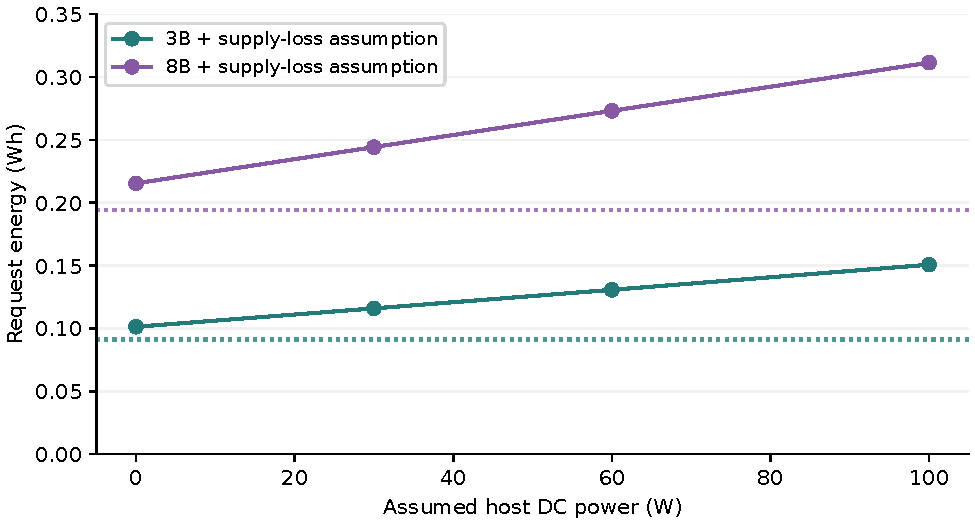
\includegraphics[width=\columnwidth]{review_energy.pdf}
\caption{Primary-session host-power sensitivity. Dotted lines are board
medians. Solid curves include assumed host power and supply loss, not
additional idle time or cooling.}
\label{fig:host}
\end{figure}

\subsection{AMD Throughput and Prefill}
\begin{table}[t]
\caption{AMD main-run decode and reconstructed prefill fits. Fitted $1/b$
is in tokens/s and $a$ in ms; $\widehat{\beta}$ is evaluated at 500 input
and 300 output tokens.}
\label{tab:amd}
\centering\small
\setlength{\tabcolsep}{4pt}
\begin{tabular}{lrrrr}
\toprule
Recorded build & Decode & $1/b$ & $a$ & $\widehat{\beta}$\\
\midrule
\ReviewAmdRows
\bottomrule
\end{tabular}
\end{table}

Decode medians are 78.4, 37.8, and 13.8 tokens/s
(Table~\ref{tab:amd}). Projected prefill/decode ratios are 0.050--0.078.
These results describe one prompt family and serving configuration, not
arbitrary agent workloads. The 27B tag has a different rate in the shorter
ladder protocol; reporting both does not make them interchangeable.

\subsection{Why the Ladder Is Not a Bandwidth Measurement}
\begin{table*}[t]
\caption{All archived ladder rows. Proxy percentages are
$100U_{\mathrm{file}}$, recomputed from stored file sizes and throughput.
Summary means the raw repetitions are unavailable.
Runtime tags identify these records, not universally reproducible weights.}
\label{tab:ladder}
\centering\small
\setlength{\tabcolsep}{9pt}
\begin{tabular}{llrrrr}
\toprule
Platform & Recorded model tag & File GB & Tokens/s & Proxy (\%) & Evidence\\
\midrule
\ReviewLadderRows
\bottomrule
\end{tabular}
\end{table*}

Table~\ref{tab:ladder} retains all nine AMD and three NVIDIA rows.
AMD proxies range from 76.7\% to 581.6\%; NVIDIA rows range from 63.1\%
to 93.2\%. Values above 100\% do not demonstrate violation of a physical
limit. They reject the interpretation that file size equals externally
transferred bytes per output token under the stated bandwidth reference.

An anonymized vision-language build reaches 105.7\%. A dense runtime
label does not imply every file byte is read from external memory per
decoded token. Likewise, an architecture metadata flag for multi-token
prediction does not prove its use or establish an acceptance rate.
The excess supplies no upper bound on proxy error for other builds.
Neither a 30-percentage-point separation between selected groups nor
high proxy values establish causal architectural classification or
universal memory-bound behavior. Hardware traffic counters and runtime
instrumentation would be needed to test those explanations.

\section{Conditional Sustainability Accounting}
\subsection{Functional Unit and Quality}
The desired functional unit is a completed task satisfying a predeclared
quality and latency requirement, including retries and fallbacks.
Token counts alone do not define that unit; different tokenizers and
answers also matter. Our timing prompt is not a quality evaluation.

For task classes $k$, let $w_k$ be deployment frequencies, $p_k$ the
fraction attempted locally, and $q_k$ the conditional probability that a
local attempt is followed by a cloud call. Let $F_{e,k}$ and $F_{c,k}$
be per-attempt footprints for metric $F$, with comparable boundaries.
If one cloud call resolves each escalation, expected footprint is
\begin{align}
D_F={}&\sum_k w_k\big[(1-p_k)F_{c,k}
+p_kF_{e,k}+p_kq_kF_{c,k}\big]\nonumber\\
&+R_F+N_F, \label{eq:routing}\\
F_0={}&\sum_k w_kF_{c,k},\qquad \sum_k w_k=1. \label{eq:baseline}
\end{align}
$R_F$ and $N_F$ are routing and additional network overhead per original
task, excluding anything already in the attempt footprints.
Multiple retries require extra terms. The $p_kq_kF_{c,k}$ term must not
be omitted merely because the final answer comes from the cloud.

In a one-class, no-failure special case,
$D_F=fF_e+(1-f)F_c+R_F+N_F$.
We do not estimate $f$, $p_k$, or $q_k$ from timing records.
The earlier assumption $f=0.82$ at relative-quality threshold 0.70 was
not a measured routing rate; allowing 70\% of a benchmark score is not
evidence of equivalent service quality.

\subsection{Carbon, Water, and Cost}
With energy in Wh and location-based grid intensity $I_j$ in
gCO$_2$e/kWh, emissions are
\begin{equation}
C_j=E_jI_j/1000+A_j, \label{eq:carbon}
\end{equation}
where $A_j$ consistently allocates non-operational emissions in
gCO$_2$e per task. Allocating fraction $a$ of hardware embodied emissions
$M$ kgCO$_2$e over $Q$ tasks gives $A=1000aM/Q$.
Allocation is not automatically consequential emissions avoided by
using existing hardware. Purchase, lifetime, and replacement
counterfactuals must be specified on both sides.
Market-based provider values must not be silently mixed with
location-based household factors.

If $E_j$ includes facility electricity, PUE is known, and both water
intensities describe consumption, operational water is
\begin{equation}
W_j=E_j\left(u_j/\mathrm{PUE}_j+v_j\right)
\quad\text{in mL}. \label{eq:water}
\end{equation}
$u_j$ is on-site L/kWh of IT electricity; $v_j$ is off-site L/kWh of
facility electricity. The factors of 1000 converting Wh to kWh and L to
mL cancel. Withdrawal must not be added to a consumption-only input
\cite{li2025water}. A zero on-site term is justified only if that boundary
has no consumptive cooling. Electricity, building cooling, and
manufacturing can still use water.

At electricity price $p_{\mathrm{elec}}$ in dollars/kWh,
\begin{equation}
K_{\mathrm{electricity}}=E_{\mathrm{AC}}p_{\mathrm{elec}}/1000.
\end{equation}
The primary 8B, 60 W-host scenario at an assumed \$0.16/kWh gives
approximately \$0.000044 per request for electricity. This excludes
equipment, maintenance, standby allocation, network charges, and labor.
It is not total cost of ownership or a quality-matched API saving.

\subsection{Rebound and Break-Even Conditions}
For a scenario with demand growth $g$, fixed task mix, and fixed
per-task footprints, the \emph{same} $g$ applies to every metric:
\begin{equation}
D_F^{\mathrm{eff}}=(1+g)D_F,\qquad
S_F=1-(1+g)D_F/F_0. \label{eq:rebound}
\end{equation}
For $0<D_F<F_0$, break-even growth is
\begin{equation}
g_F^*=F_0/D_F-1. \label{eq:gstar}
\end{equation}
If $D_F\ge F_0$, there is no saving at nonnegative growth.
Thresholds differ by metric because footprints differ, not because one
scenario can have different query-volume growth for water and carbon.

A numerical unit check does not assert deployment parameters.
Set $F_c=1$, $F_e=0.25$, $p=0.80$, $q=0$, and overhead zero.
Then $D_F=0.40$ and $g=0.25$ gives $S_F=0.50$; break-even is
$g^*=1.50$. If 10\% of local attempts also invoke the cloud
($q=0.10$), $D_F=0.48$ and savings at the same growth fall to 0.40.

A take-back fraction $r$ satisfies
$g=r(F_0-D_F)/D_F$ for a \emph{single} metric with positive gross saving.
Applying one $r$ separately to energy, water, and carbon generally implies
different $g$ values, not one physical demand scenario. No observed
elasticity is available here; rebound is not empirically refuted.

\subsection{Why We Do Not Report a Cloud-Savings Percentage}
The 0.24 Wh Gemini median is a production-population measure with a
broader boundary \cite{elsworth2025}.
GPT-4o short and long estimates of 0.421 and 1.788 Wh are version-specific
values from Jegham et al., v3, Table 4 \cite{jegham2025}.
Their workload definitions are 100/300 and 10\,000/1500 input/output
tokens. Neither supplies a quality-matched 499/300-token cloud
counterfactual for these builds. Linear token-count normalization would
ignore prefill, decode, caching, batching, and reasoning differences.

Google's comprehensive breakdown includes host and infrastructure costs.
Their existence does not mean a desktop removes them: it also has host
and supply costs. Using a global grid factor does not reproduce a
provider's reported market-based carbon footprint.

Multiplying 945 TWh by assumed AI share, inference share, adoption, and a
mismatched per-query reduction does not establish an IEA-backed
fleet-saving forecast. It needs workload-weighted energy shares and
displacement evidence. Monte Carlo over selected priors cannot supply
that evidence; favorable simulation draws are not a measured probability
that a deployment will save resources.

\section{Transport and System Scope}
WebRTC data channels use SCTP over DTLS \cite{rfc8831}.
An ordinary TURN relay forwards encrypted traffic and need not receive
application plaintext, provided endpoint authentication and signaling
integrity hold. The security architecture distinguishes passive protection
from an active attack through compromised or untrusted signaling
\cite{rfc8827}. An inference peer can read the prompt, as can a remote
router that classifies it. Encryption does not remove metadata exposure
or endpoint trust.

These are protocol considerations, not an implementation security audit.
There is no measured network-energy experiment, relay probability study,
or P2P-versus-cloud session trial here. We include network and routing as
unmeasured terms in Eq.~\eqref{eq:routing}, without a numerical
transmission-saving claim.

\section{Limitations and Required Experiments}
The strongest supported claim is narrow: the traces are internally
consistent and describe short, warm, single-stream runs on the stated
stacks. Major limits remain.

\emph{External validity.} Two machines, a synthetic prompt family, small
repetition counts, and fixed output limits do not represent an assistant
workload. Same-machine repeats do not establish cross-machine or
independent reproducibility. Software, thermal state, clocks, model format,
and batching can change results. Runtime tags can change; immutable
digests and retrieval instructions are needed for full build reconstruction.

\emph{Measurement validity.} Board telemetry is not wall energy.
There is no external-meter calibration or systematic sensor-error interval.
Run ranges omit shared systematic errors. Auxiliary prompt sweeps and
all AMD ladder rows lack their individual observations in this archive.

\emph{Service validity.} There is no matched quality evaluation, routing
confusion matrix, success/fallback trace, or representative task distribution.
We cannot infer that parameter count alone determines capability, that all
large local models lose to cloud serving, or that fine-tuning changes
coverage by a known amount. The companion adaptation manuscript is
outside this experiment.

The next decisive experiment would use a released, held-out task set with
prespecified quality and latency thresholds. It would measure the same
tasks on local and cloud alternatives, log failed attempts and retries,
calibrate longer wall-meter runs against telemetry, and separate cold,
active, and keep-awake energy. Multiple sessions and machines, randomized
order, and thermal/clock records would improve uncertainty analysis.
Cloud energy needs a cooperating provider's instrumentation or explicit
identification as an estimate; client API timing cannot measure provider
power.

\section{Reproducibility and Research Integrity}
The original harness and supplied records are in the public research
repository \cite{autoyou2026measure}. The accompanying revision artifact
adds \texttt{review/audit.py}, synthetic unit tests, a JSON report, and
SHA-256 hashes of all six input files.
Replay requires no live model, cloud credentials, private logs, or personal
user data. It generates the numerical macros used by this manuscript and
the host-sensitivity figure. From the research repository, run:
\begin{quote}\small
\texttt{python review/audit.py}\\
\texttt{python -m unittest discover -s review}\\
\texttt{python -m unittest measure.test\_bench}\\
\texttt{python review/build\_paper.py}
\end{quote}
Figure generation requires \texttt{requirements.txt}.
Legacy scenario generators and the companion manuscript are retained for
provenance, but are not the validation path for these revised results.

An AI assistant assisted this revision with source checking, arithmetic
replay, code, and drafting. This is not independent peer review or laboratory
replication. Authors remain responsible for the measurements,
interpretation, rights, authorship, and final submission declarations.

\section{Conclusion}
The records support a reproducible, boundary-limited consumer-inference
case study. For the 499/300-token RTX 5070 experiment, board telemetry yields
medians of 0.091 and 0.19 Wh; host and supply assumptions materially increase
system estimates. File-size throughput ratios cannot establish actual
bandwidth utilization. A credible sustainability comparison must additionally
measure equivalent task quality, failed local attempts, fallback, and
comparable boundaries. Right-sizing remains a testable deployment hypothesis,
not a quantified environmental benefit established by these records alone.

\bibliographystyle{IEEEtran}
\IEEEtriggeratref{8}
\bibliography{review_references}
\end{document}
